\section{Dockerを使用した深層学習アプリケーションのデプロイ(Ollamaを例に)}
Ollamaは、多様なオープンソースの大規模言語モデル(LLM)を提供するプラットフォームであり、ユーザーは必要なモデルを検索、ダウンロード、実行できます。また、Open WebUIは、拡張性が高く、ユーザーフレンドリーな自己ホスティング型AIプラットフォームであり、完全オフラインで動作可能です。本システムは、OllamaやOpenAI互換APIを含む様々なLLM環境をサポートし、検索拡張生成(Retrieval-Augmented Generation, RAG)用の推論エンジンを内蔵しています。これは強力なLLMアプリケーションのデプロイソリューションとなります。

\subsection{NVIDIA Container Toolkitのインストール}
新規インストールされたDockerでは、NVIDIAのCUDAデバイスを直接利用できません。しかし、多くの深層学習およびAIアプリケーションでは、CUDAランタイムライブラリおよびデバイスが必要となります。そのため、\texttt{NVIDIA Container Toolkit}をインストールする必要があります。

まず、NVIDIAドライバが正常にインストールされていることを確認します。
\begin{lstlisting}[language=bash]
nvidia-smi
\end{lstlisting}

次に、\texttt{NVIDIA Container Toolkit}をインストールします。
\begin{lstlisting}[language=bash]
# NVIDIA公式GPGキーを追加
curl -fsSL https://nvidia.github.io/libnvidia-container/gpgkey | sudo gpg --dearmor -o /usr/share/keyrings/nvidia-container-toolkit-keyring.gpg \
  && curl -s -L https://nvidia.github.io/libnvidia-container/stable/deb/nvidia-container-toolkit.list | \
    sed 's#deb https://#deb [signed-by=/usr/share/keyrings/nvidia-container-toolkit-keyring.gpg] https://#g' | \
    sudo tee /etc/apt/sources.list.d/nvidia-container-toolkit.list

# nvidia-container-toolkitのインストール
sudo apt-get update
sudo apt-get install nvidia-container-toolkit
\end{lstlisting}

\subsection{OllamaとOpen WebUIのDockerイメージを使用したデプロイ}
Open WebUIはOllamaと統合されたDockerイメージを提供しており、簡単にデプロイ可能です。

以下のコマンドを実行します。
\begin{lstlisting}[language=bash]
docker run -d --gpus=all \
  -p 11919:8080 \
  -v ollama:[your path]/ollama-model \
  -v open-webui:[your path]/openwebui-data \
  --name open-webui-ollama \
  --restart always \
  ghcr.io/open-webui/open-webui:ollama
\end{lstlisting}

パラメータの説明:
\begin{itemize}
  \item \texttt{run}: コンテナを実行します。コン테ナの起動コマンドとして使用します。
  
  \item \texttt{-d}: バックグラウンドで実行します。サービス指向型アプリケーションに推奨されます。
  
  \item \texttt{--gpus=all}: 全てのGPUアクセスを許可します。GPUを使用する場合に必要です。
  
  \item \texttt{-p 11919:8080}: ポートをマッピングします。安全なため、一般的なポート(8080)を避けています。
  
  \item \texttt{-v ollama:/root/.ollama}: モデルを永続化します。\\ \texttt{/var/lib/docker/volumes/ollama\_data}にデータが保存されます。
  
  \item \texttt{-v open-webui:/app/backend/data}: ユーザーデータを永続化します。会話履歴やカスタム設定が保存されます。
  
  \item \texttt{--restart always}: コンテナの自動再起動を設定します。コンテナ障害時に復旧します。
  
  \item \texttt{ghcr.io/open-webui/open-webui:ollama}: 使用するイメージを指定します。信頼できるソースの使用推奨。
\end{itemize}

コンテナが正常に起動すると、\texttt{http://localhost:11919} にアクセスできます。

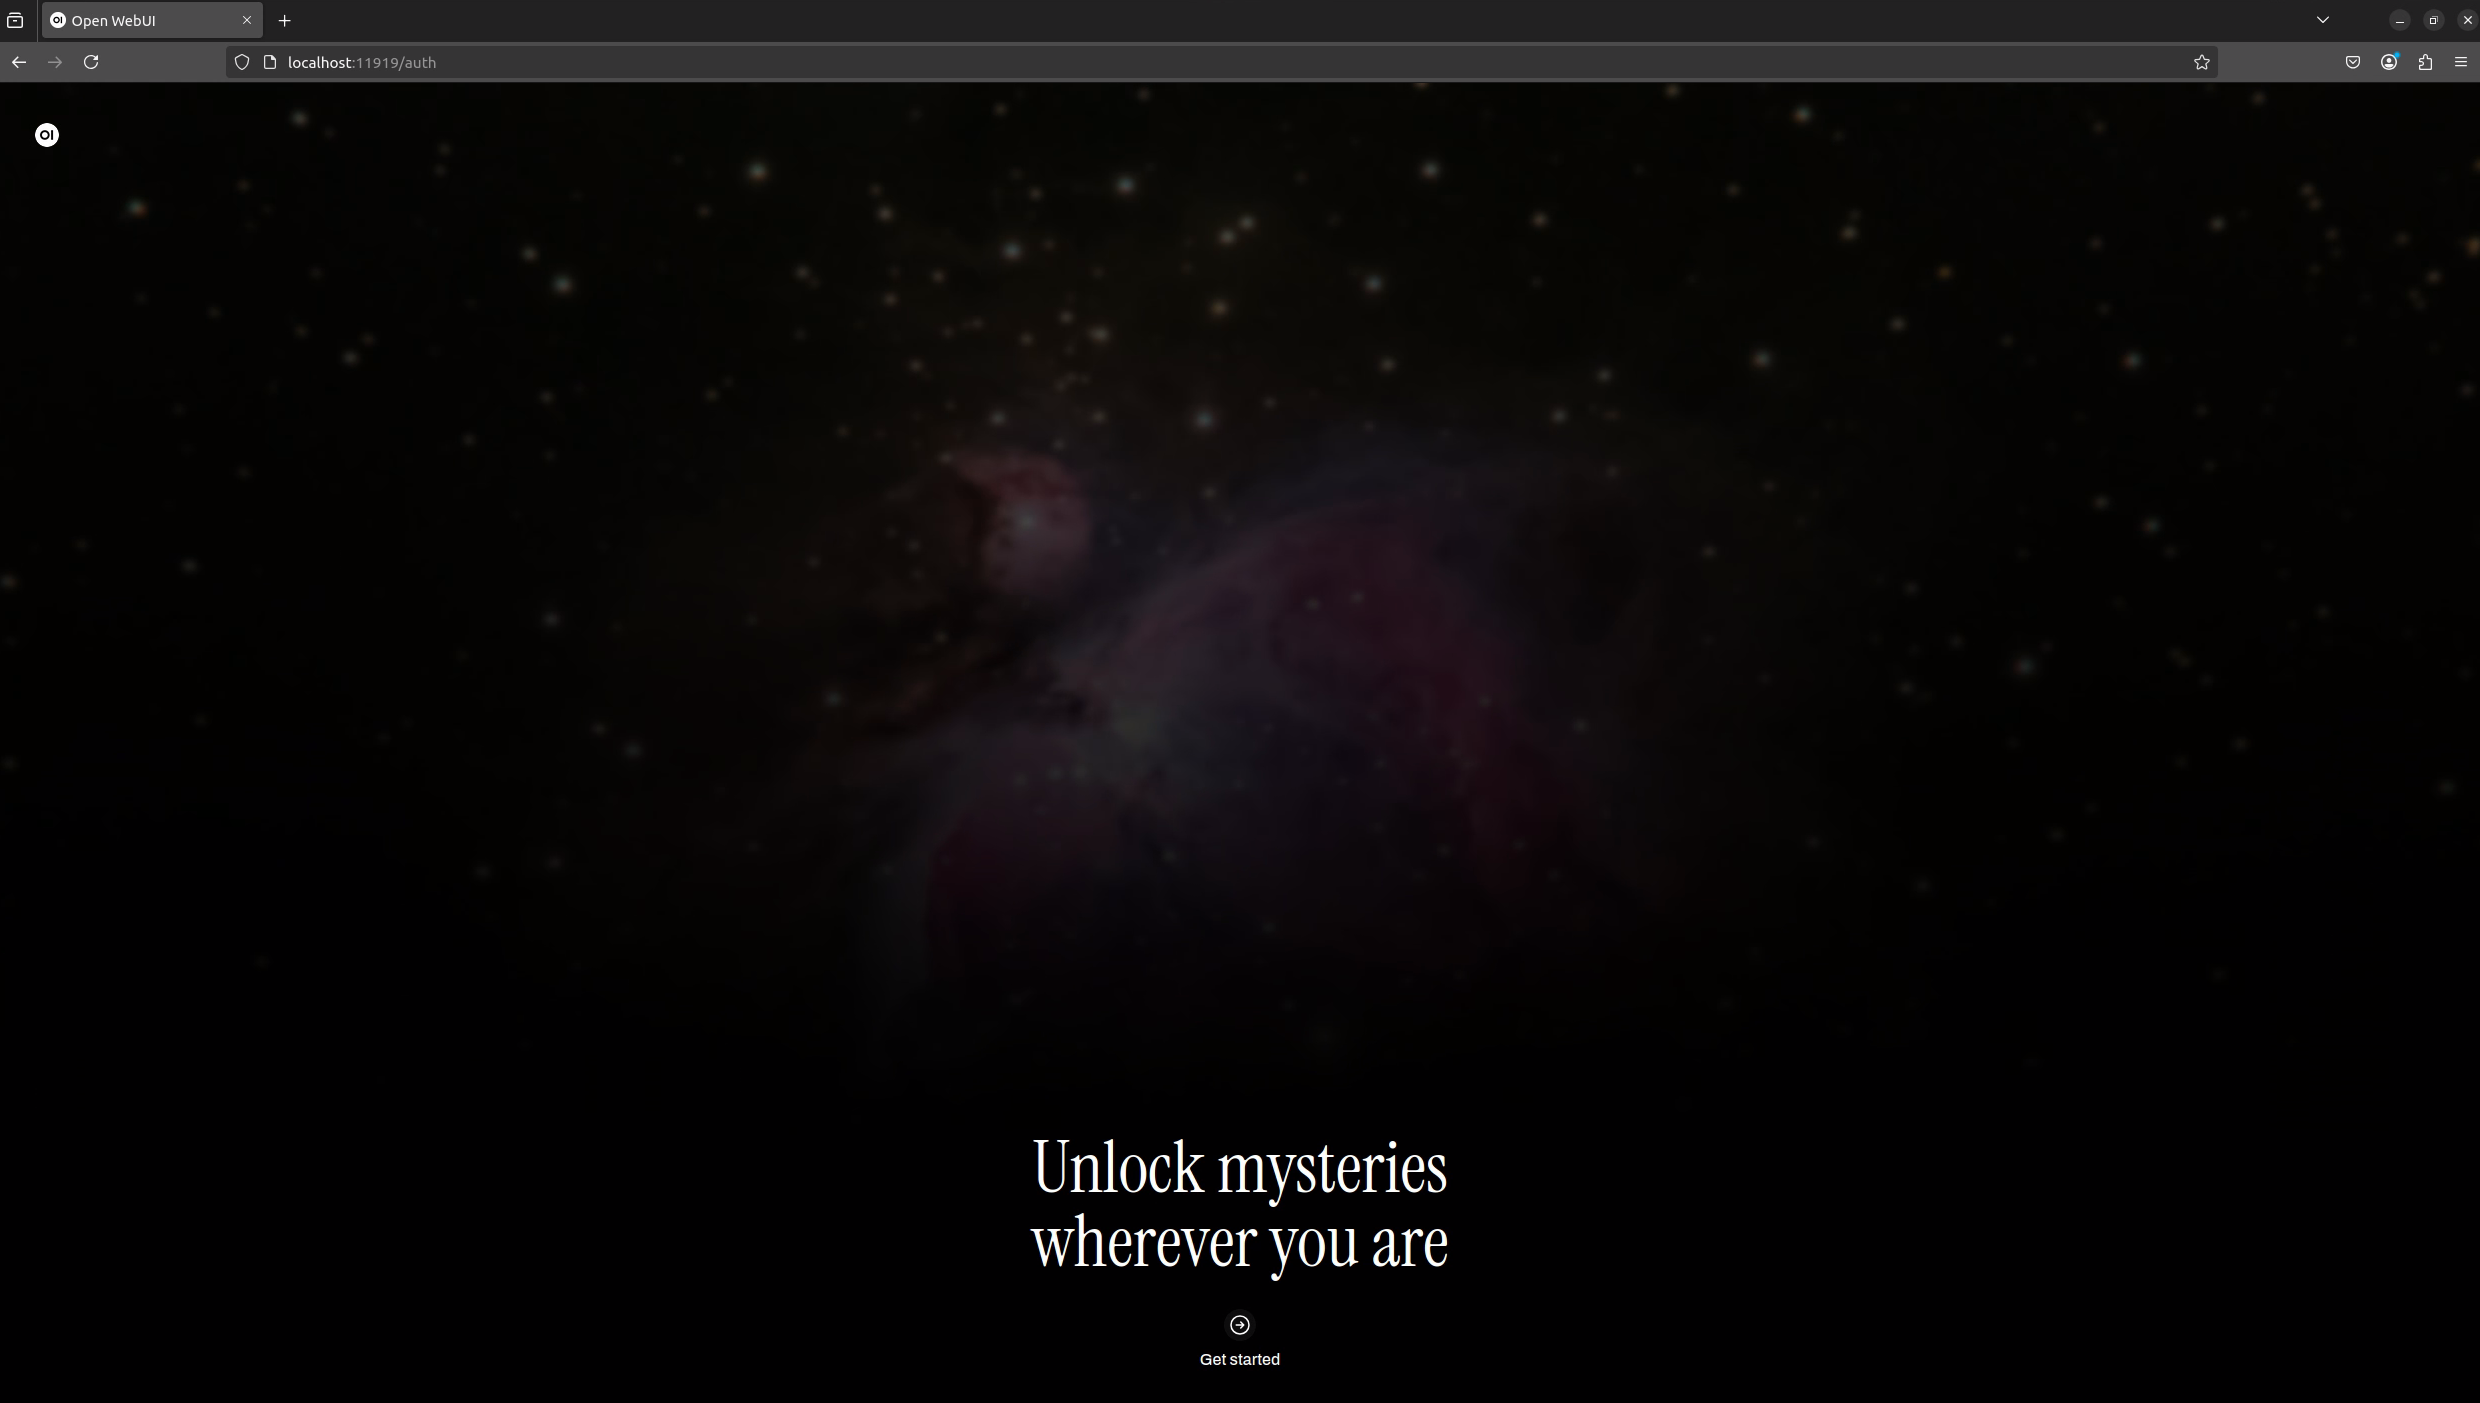
\includegraphics[width=0.8\linewidth]{images/Pasted image 20250304171521.png}

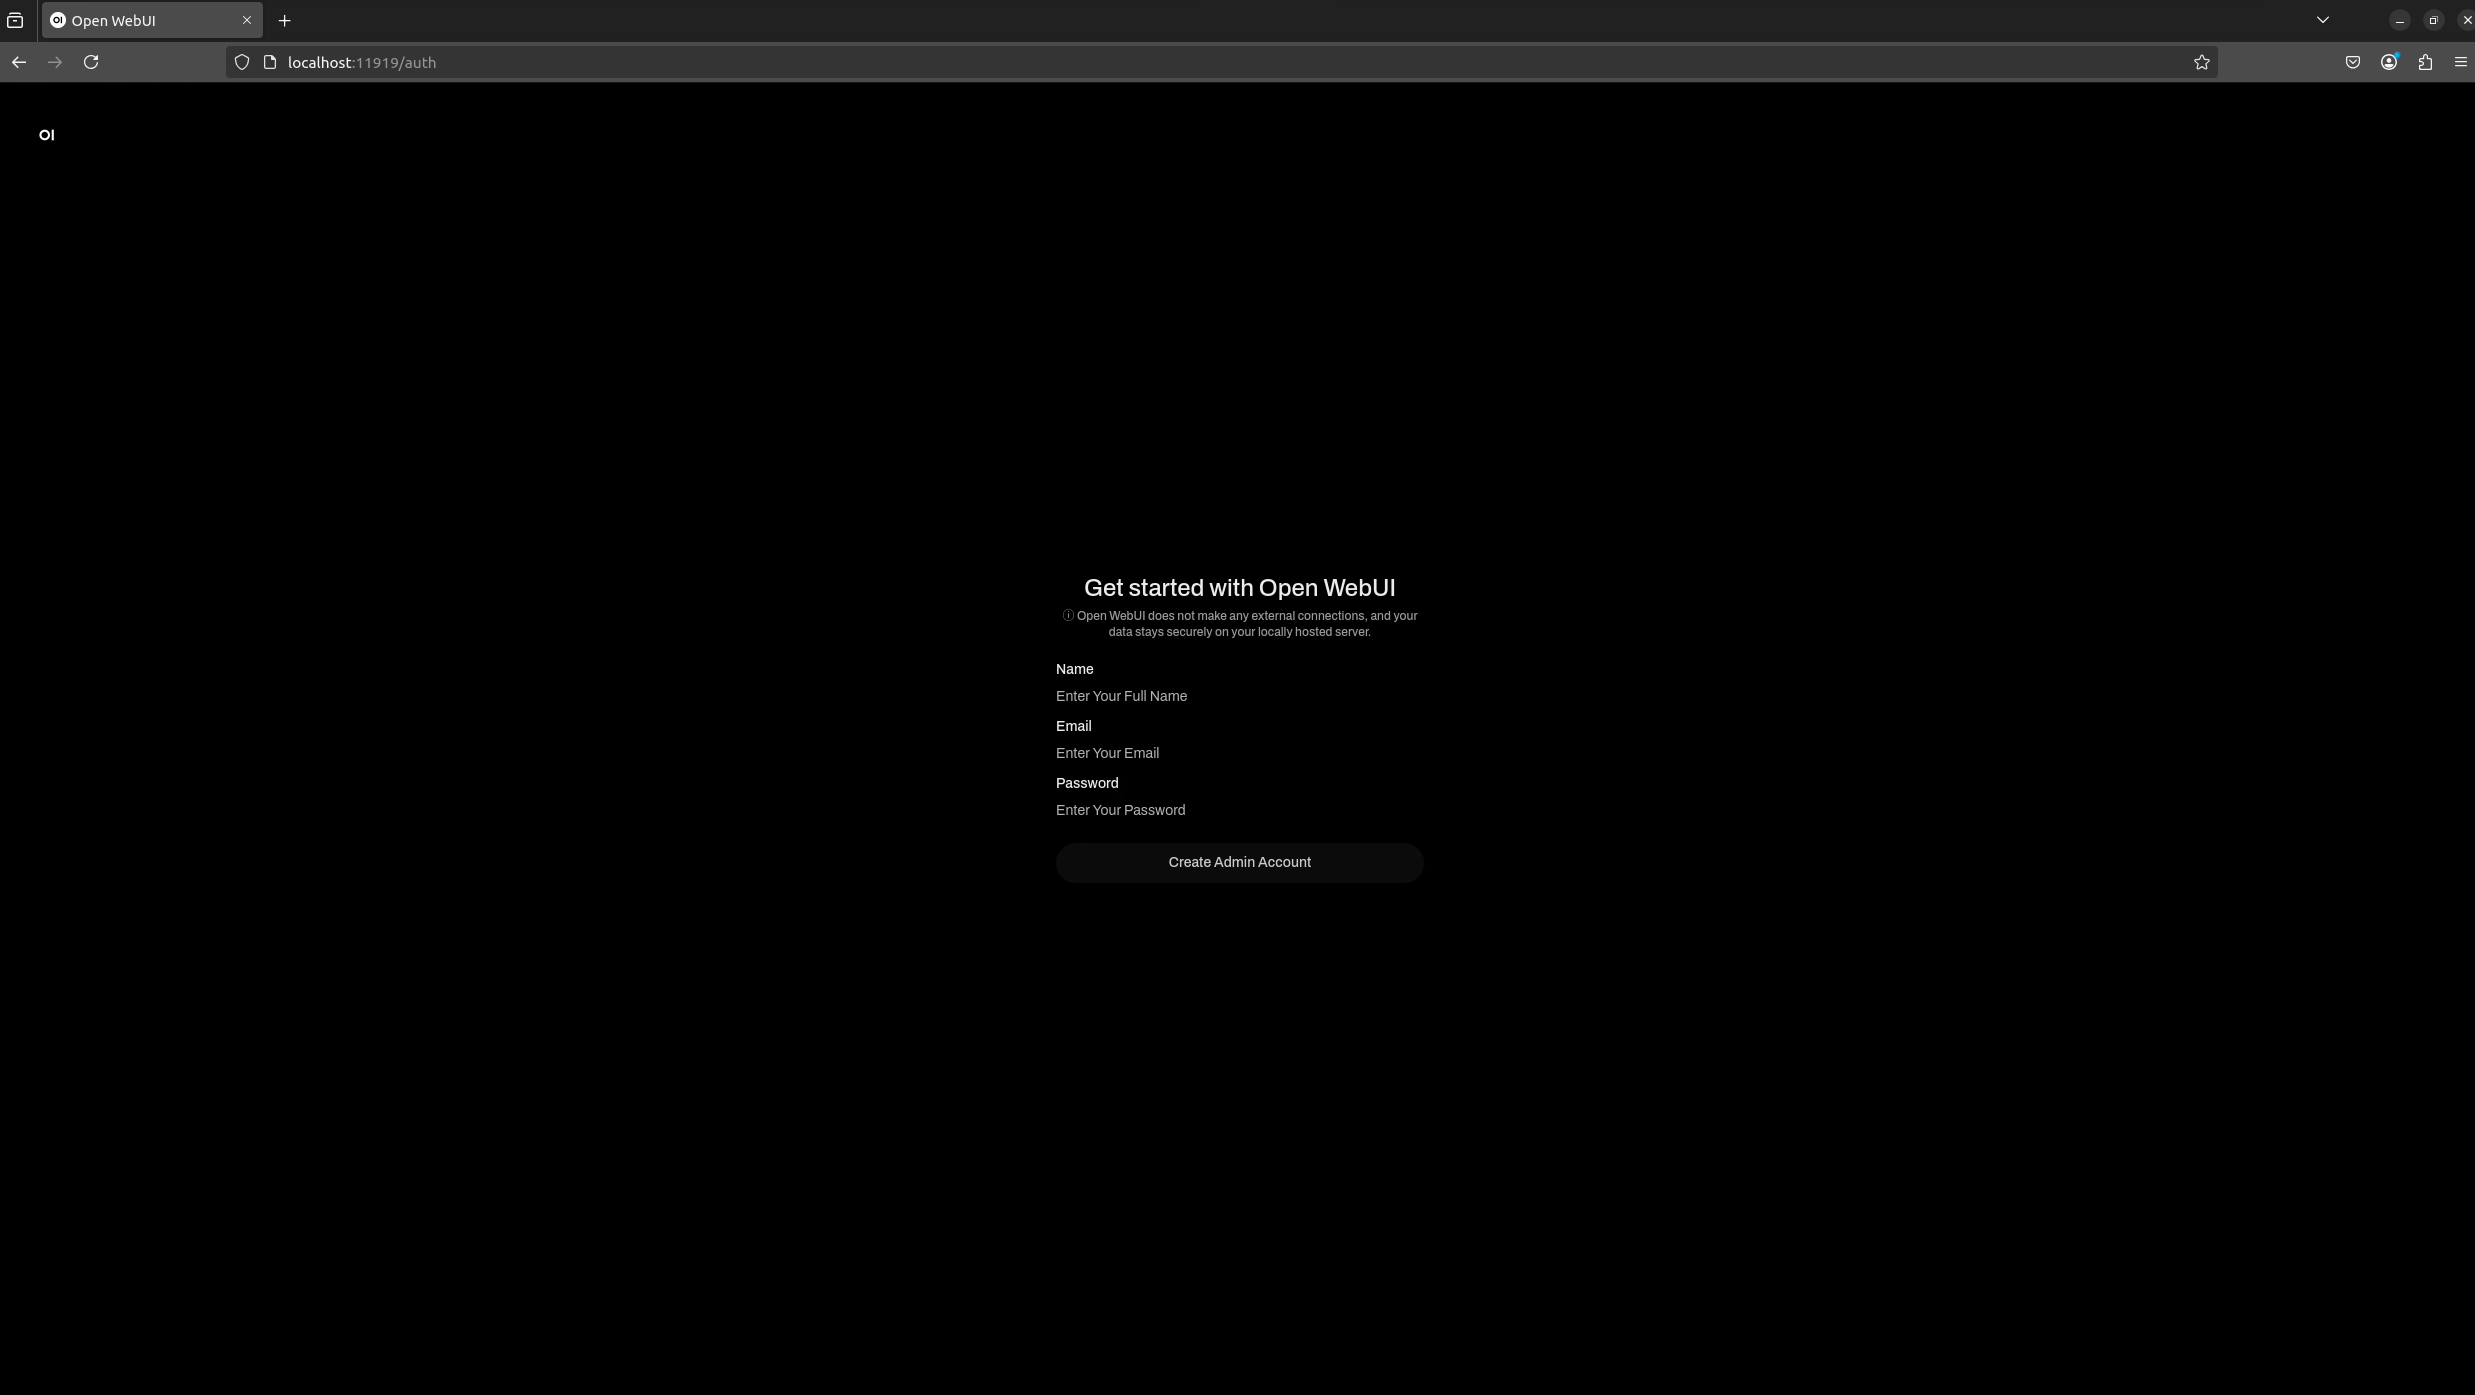
\includegraphics[width=0.8\linewidth]{images/Pasted image 20250304171548.png}

ログインすると、以下の画面が表示されます。

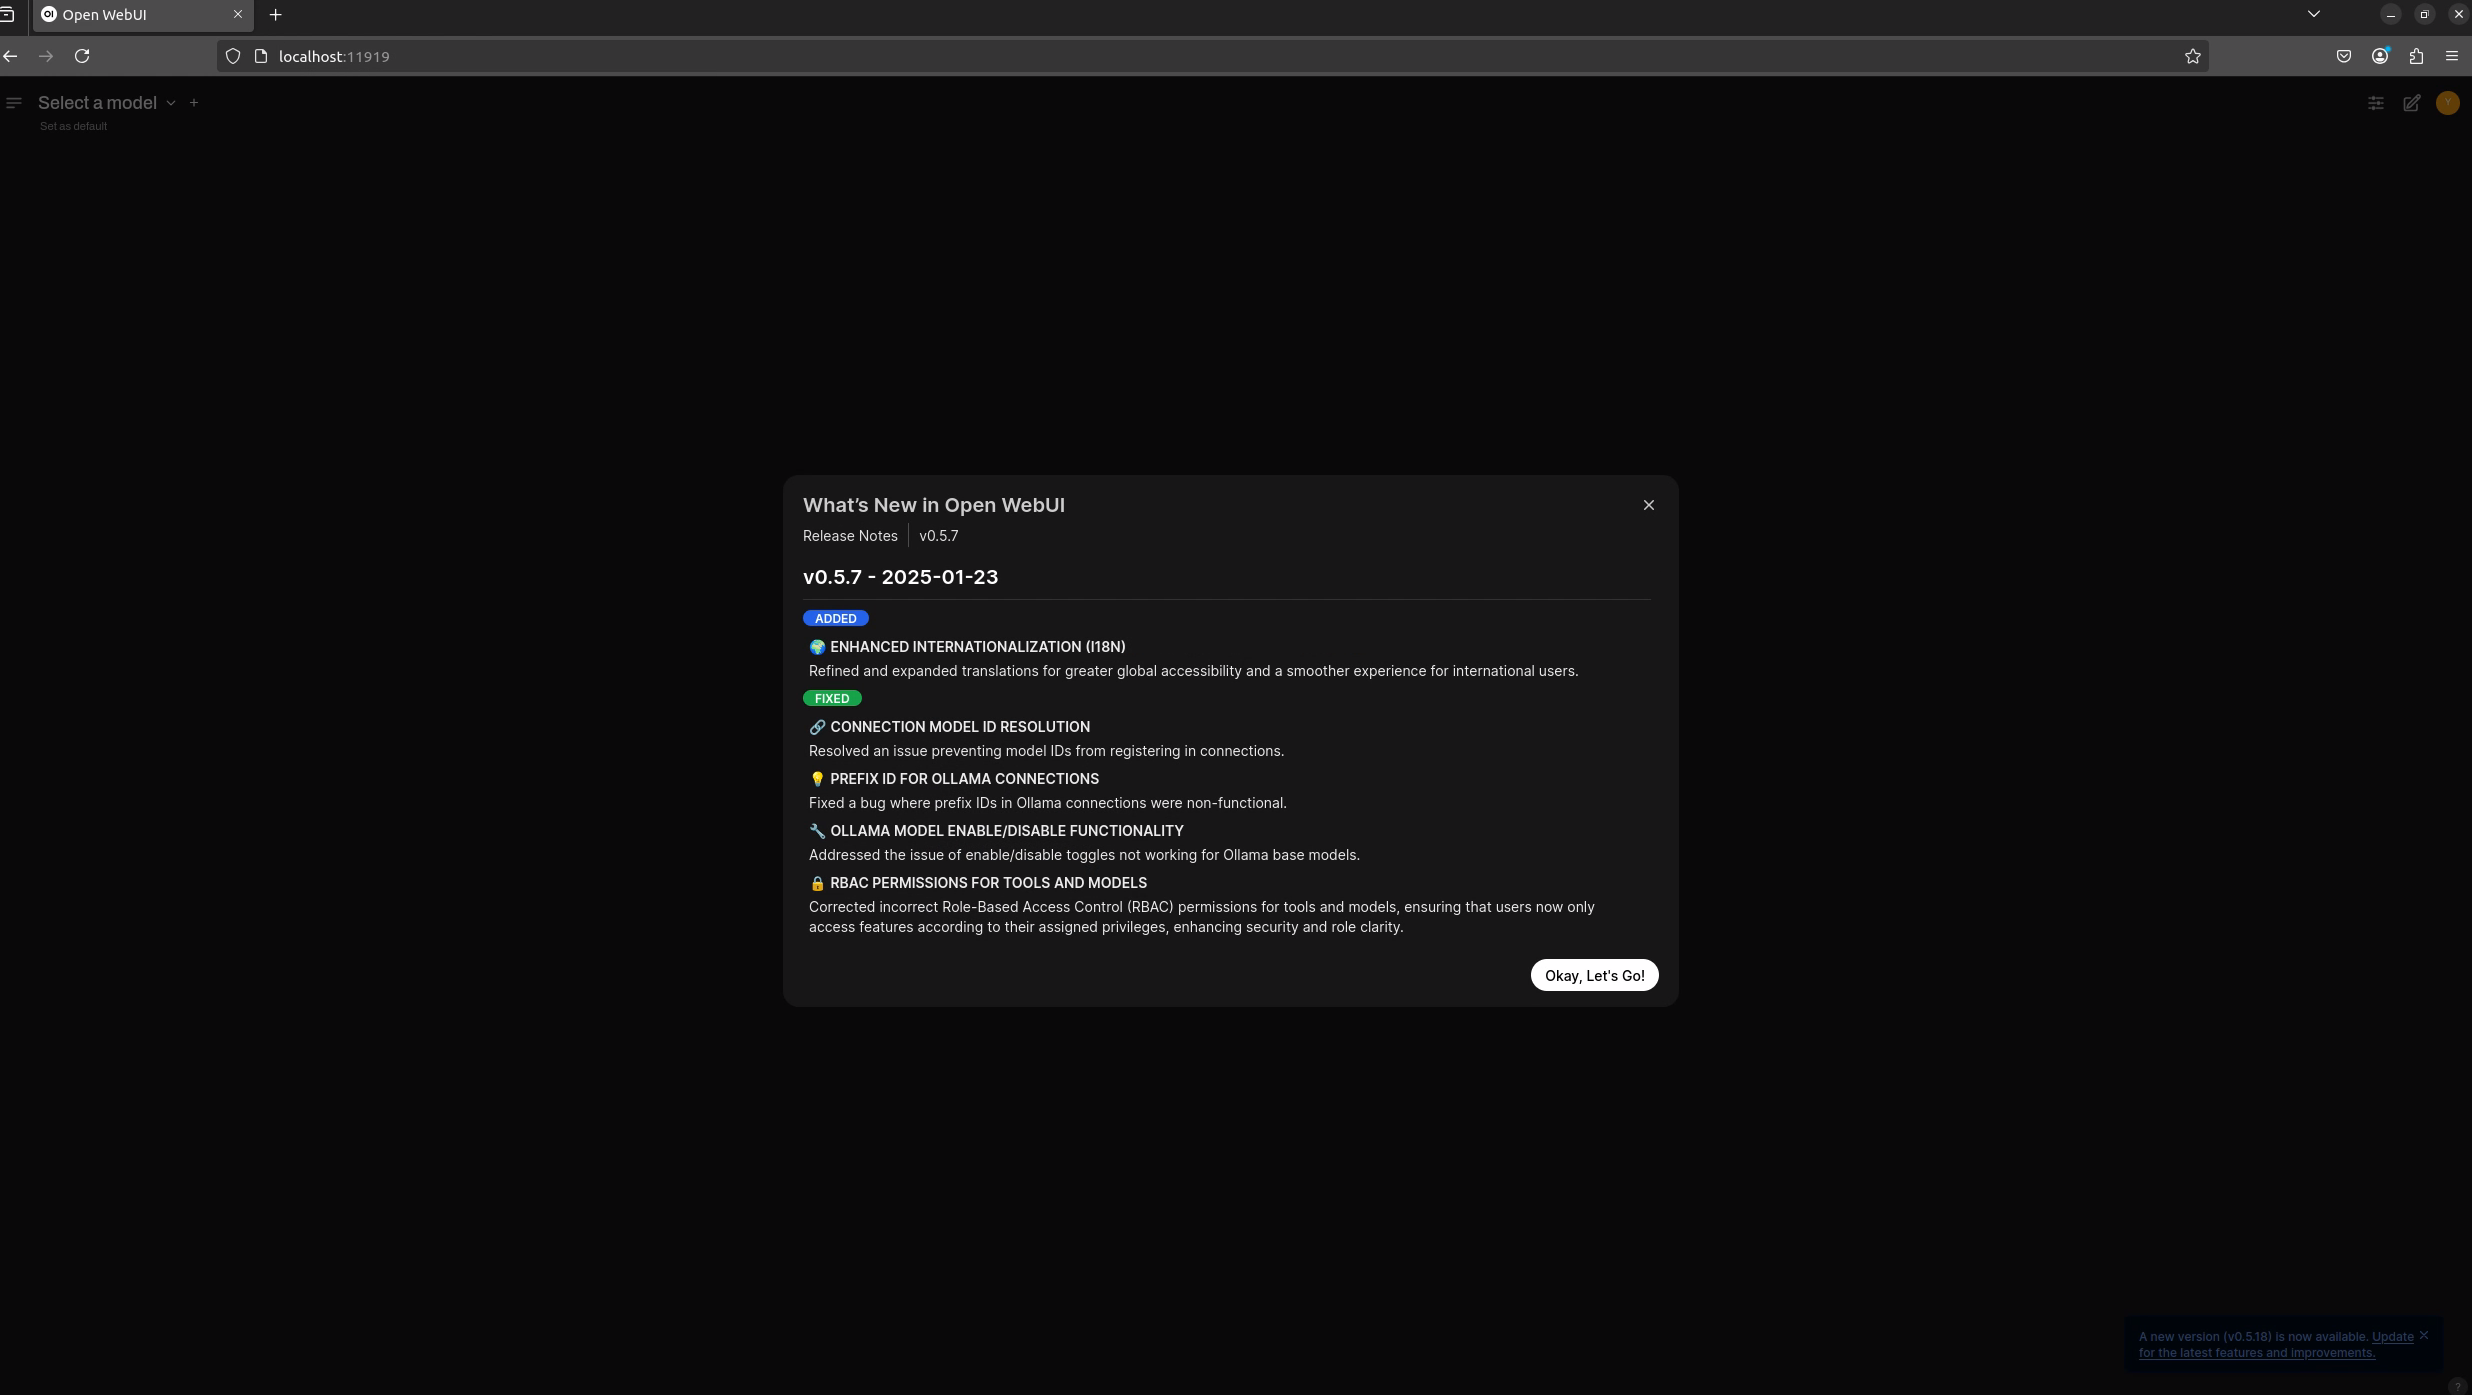
\includegraphics[width=0.8\linewidth]{images/Pasted image 20250304171722.png}

この時点では、モデルリストは空です。

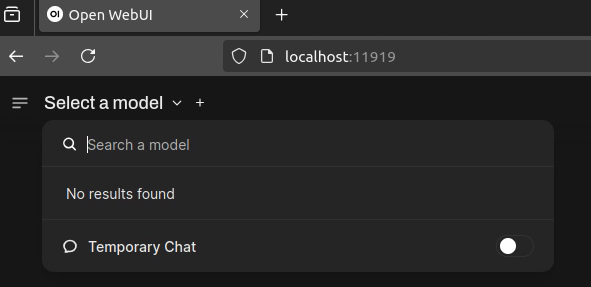
\includegraphics[width=0.8\linewidth]{images/Pasted image 20250304171753.png}

\paragraph{注意} 長時間GPUを使用しない場合、NVIDIAのドライバがGPUとの接続を自動で切断し、推論速度が大幅に低下することがあります(CPU推論に切り替わる)。その際は、以下のコマンドでコンテナを再起動してください。
\begin{lstlisting}[language=bash]
docker restart open-webui-ollama
\end{lstlisting}

\section{ローカルでのOpen WebUIの使用}
Ollamaがサポートするモデルは、\href{https://ollama.com/search}{公式ページ}で検索できます。例えば、`deepseek-r1:14b` モデルを使用する場合、以下のコマンドで実行できます。
\begin{lstlisting}[language=bash]
docker exec -it open-webui-ollama ollama run deepseek-r1:14b
\end{lstlisting}

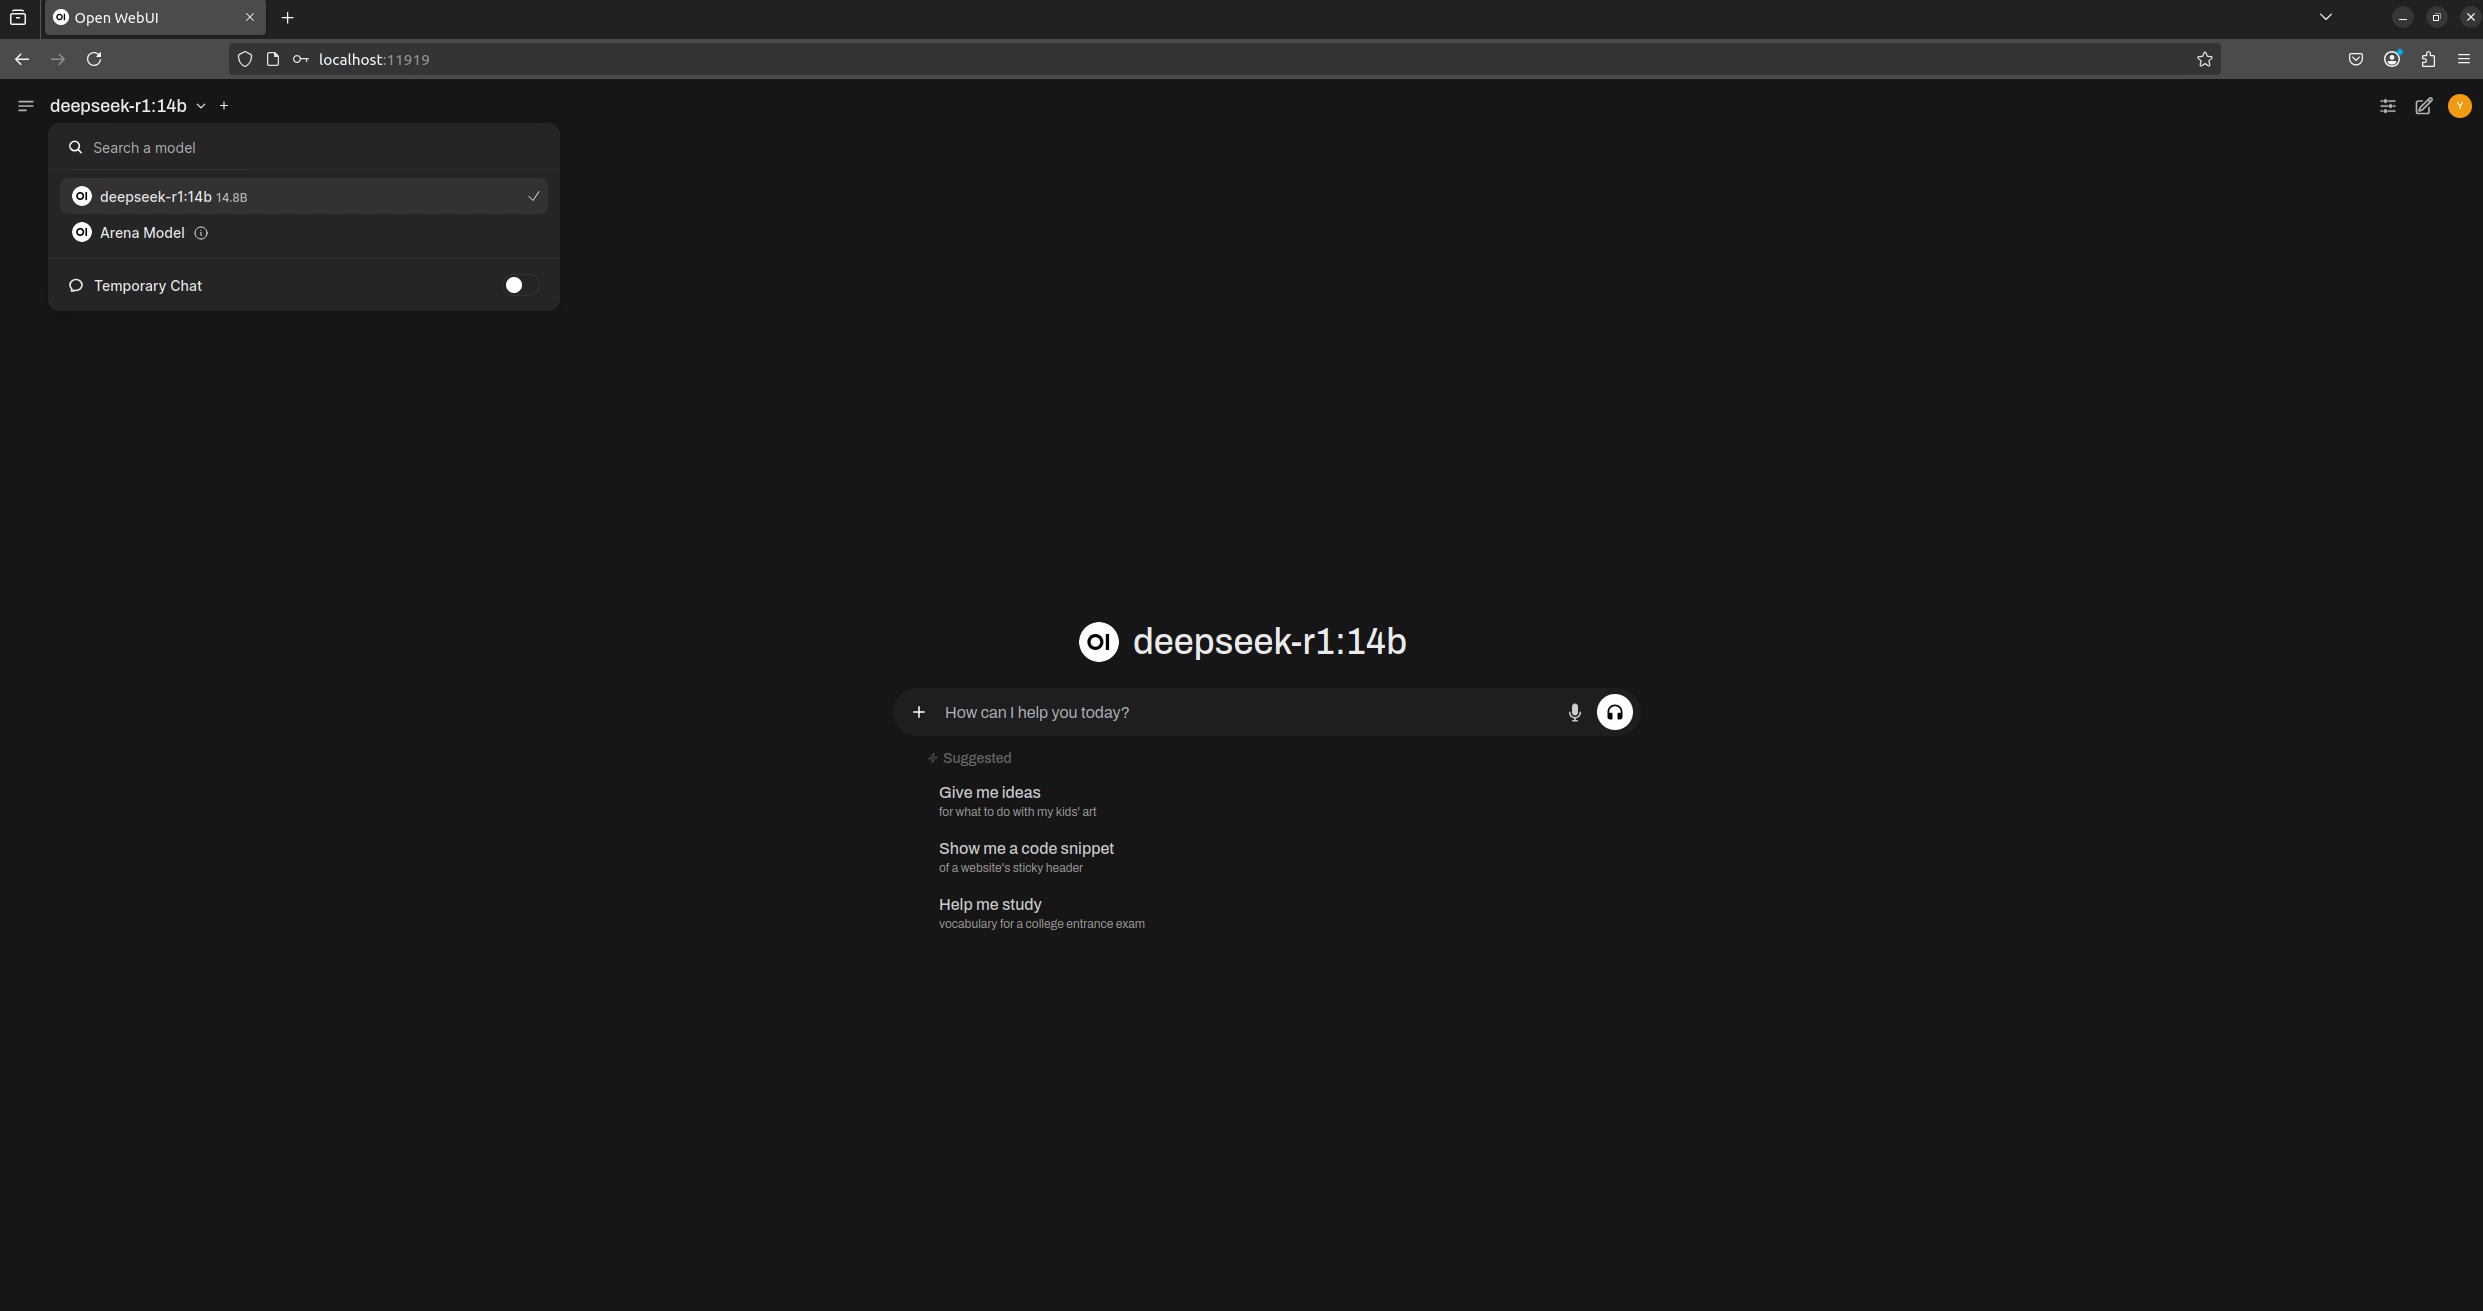
\includegraphics[width=0.8\linewidth]{images/Pasted image 20250304170628.png}

右上のモデルパラメータから、各種パラメータの微調整も可能です。ユーザーのさらなる活用を期待します。